\chapter{Metodología}

A continuación se describe detalladamente la metodología que se ha llevado a cabo para el cumplimiento de los objetivos del proyecto de investigación. En cada actividad también se describen los resultados preliminares obtenidos.

\section{Diseño y calibración del sistema electrónico del hodoscopio}

Para la medición del flujo de partículas dependiendo de la trayectoria se desarrollará un hodoscopio con dos paneles compuestos de 60 centelladores plásticos cada uno. Cada centellador tendrá un SiPM S13360-6050CS como elemento sensor. Las señales de cada panel serán discriminadas mediante un sistemas de adquisición (DAQ) basado en el Circuito de Aplicación Específica (ASIC) MAROC3A para luego ser almacenadas. El sistema DAQ es controlado por un computador embebido Rapsberry Pi. El hodoscopio tendrá un sistema de disparo estratificado que determinará la veracidad de los eventos detectados y las coincidencias entre los paneles que lo conforman. \\

Por otro lado, los SiPM serán caracterizados con el fin de determinar su comportamiento (ganancia y ruido) dependiendo de la temperatura y el voltaje de ruptura. La atenuación de la señal en las barras centelladoras será medida para diferentes puntos de interacción usando un sistema de estimulación controlado. Adicionalmente, se evaluará la respuesta de los paneles centelladores y el hodoscopio midiendo el flujo de muones atmosféricos en diferentes direcciones. Los resultados preliminares y detalles técnicos de las actividades relacionadas con este objetivo se muestran a continuación.\\


\textbf{Actividades y resultados preliminares}\\

\subsection{Diseño del hodoscopio}

El hodoscopio está formado por dos paneles sensibles compuestos de $30 \times 30$ barras centelladoras rectangulares de $120 \textrm{cm} \times 4 \textrm{cm} \times 1 \textrm{cm}$.\\

Los centelladores, fabricados por Fermilab, están hechos de poliestireno (Dow Styron $663$) con un recubrimiento externo de TiO$_2$ de 0.25 mm de espesor. Los dopantes del material primario son $1\%$ PPO  y $0.03 \%$ POPOP, con un pico máximo de emisión en 420 nm \cite{Anghel2015} y un tiempo de decaimiento de 1.6 ns \cite{Kleinknecht2005}. \\

Cada barra centelladora tiene un agujero de 1.8 mm de diámetro en su parte central donde va situada una fibra óptica de corrimiento de longitud de onda (WLS). En este caso se usa la fibra Saint-Gobain BCF-92 con un diámetro de 1.2 mm, un índice de refracción en el núcleo de 1.42, un pico de absorción de 410 nm y un pico de emisión de 492 nm \cite{Kuraray2018}.\\

En este caso se usa el SiPM Hamamatsu S13360-6050CS como elemento sensor. El SiPM tiene un área fotosensible de 
$1.3 \times 1.3 \textrm{mm}^2$, 667 píxeles, un factor de llenado 74$\%$, un voltaje de ruptura de 53$\pm$5 V (25 $^{\circ}$C), una ganancia de $10^5$ a $10^6$ y una eficiencia de foto-detección de  40$\%$ a 450 nm.\\

Los SiPM están acoplados de manera directa con la fibra óptica mediante un sistema mecánico anclado a la barra centelladora. Este sistema centra el extremo de la fibra óptica con la región sensible del SiPM. Ver Fig. \ref{SiPM_WLS}. Usualmente se utiliza resina óptica EJ200 de Eljen Technology para acoplar el SiPM y la fibra óptica, sin embargo, resultados de la simulación del centellador-fibra-SiPM en GEANT4 \cite{Vasquez2018} demuestran que su uso no aumenta el número de fotones que llegan al SiPM.

\begin{figure}[h!]
\begin{center}
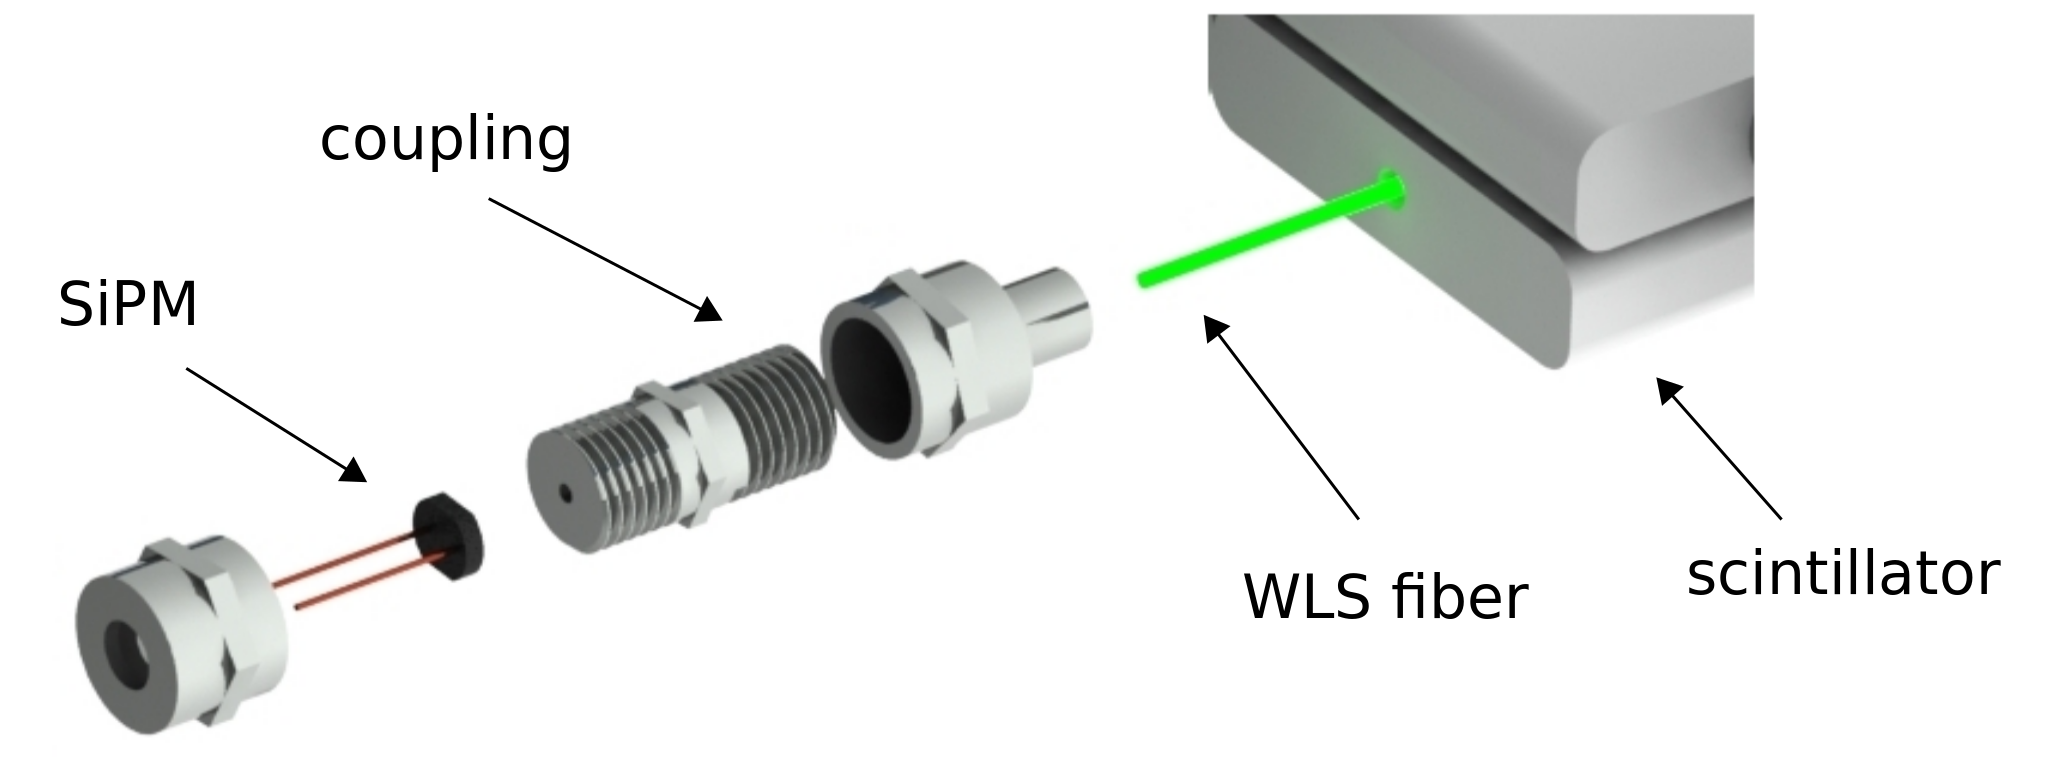
\includegraphics[width=0.7\textwidth]{Figures/panel_frontend.png}
\caption{Sistema de acople entre la fibra WLS y el SiPM en cada barra centelladora.}
\label{SiPM_WLS}
\end{center}
\end{figure}

\subsection{Diseño de la electrónica del SiPM}

 La electrónica de acondicionamiento consta de una etapa de polarización del SiPM, una etapa de amplificación (con ganancia 94) y un acople de impedancias como se muestra en Fig. \ref{SiPM_Ele}. 
 
 El circuito de polarización alimenta el SiPM con un voltaje (HV) que varia entre 40V y 80V. La fuente HV se basa en el módulo controlable C11204 de Hamamatsu.
 
 \begin{figure}[h!]
\begin{center}
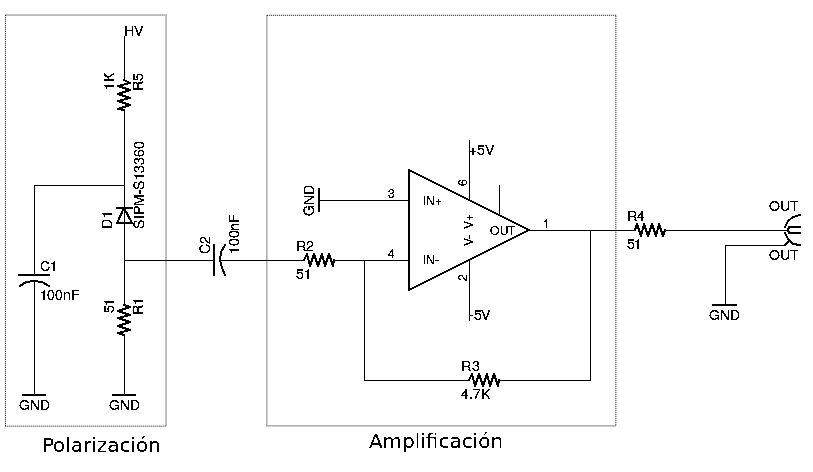
\includegraphics[width=0.7\textwidth]{Figures/Acondicionamiento.png}
\caption{Electrónica de polarización y acondicionamiento del SiPM.}
\label{SiPM_Ele}
\end{center}
\end{figure}

La fuente HV se basa en el módulo controlable C11204 de Hamamatsu el cual puede proporcionar voltajes entre 40V y 80V. Por otra parte, la amplificación de la señal pulsada se hace mediante el amplificador operacional OPA691 de Texas Instruments cuyo ancho de banda es 190 MHz. Finalmente, la señal amplificada se transmite a través de un cable coaxial RG178U con impedancia de 50 ohmnios y ancho de banda de 900 MHz.

\subsection{Diseño del sistema de adquisición del hodoscopio}

El sistema de adquisición se basa en el Circuito Integrado de Aplicación Específica (ASIC) MAROC3A de Omega, desarrollado para aplicaciones en detectores de partículas.

\begin{figure}[h!]
\centering
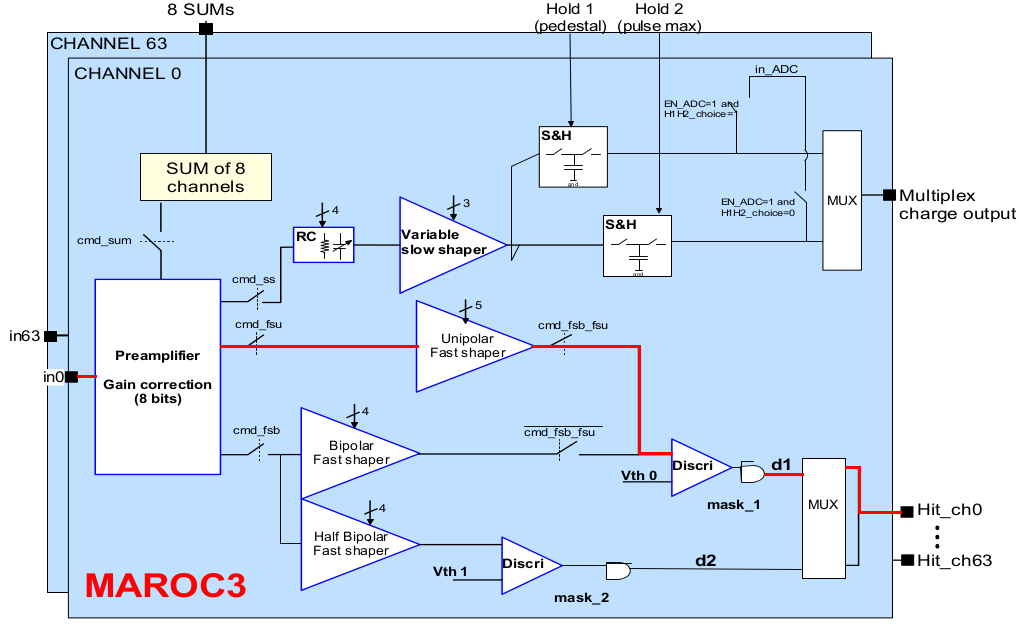
\includegraphics[scale=0.5]{Figures/Maroc.png}
\caption{Architectura del ASIC MAROC3A. La línea roja indica las etapas que recorre cada señal hasta su discriminación.}
\label{Maroc}
\end{figure}


La MAROC3A tiene 64 canales de lectura con una impedancia de entrada de 50 ohmios. Cada canal tiene una etapa de amplificación de ganancia programable (0-4), un \textrm{fast-shaper} unipolar con ganancia de 2.3V/pC y un discriminador (d1) con un umbral de discriminación ($V_{th0}$) establecido por un Convesor Digital-Análogo (DAC) de 10 bits (2.3 mV/UDAC). En la Fig. \ref{Maroc} se muestra el hilo que sigue un canal en la MAROC3A.\\

En este caso se usan solamente 60 de los 64 canales. Las señales son transportadas desde el panel centellador a través de cables coaxiales RG178U con impedancia de 50 ohmios y ancho de banda de 900 MHz. Todos los cables tienen la misma distancia (2.9 m) para evitar diferencias temporales entre canales.\\

Los parámetros de configuración de: la ganancia de amplificación, el umbral de discriminación, la elección de los $shapers$ y los discriminadores, así como la habilitación/des-habilitación de canales se hace a través de una FPGA Cyclone III de Altera. Esta información se transmite a la MAROC3A en una trama de 829 bits.\\

Los datos resultado de proceso de discriminación se ordenan en un vector de 8 bytes (64 bits - 64 canales). Cada bit toma el valor "1" si la señal de dicho canal supera el umbral de discriminación, sino toma el valor "0". Simultáneamente, cuando ocurre un evento en alguno de los 64 canales, se genera una señal de disparo (OR-Trigger o T1).\\

La adquisición de eventos en cada panel es controlada por un computador embebido (Raspberry Pi 2 - SCB) el cual almacena los datos y meta-datos de cada panel. Los datos contienen la información de las barras disparadas, el tiempo de ocurrencia del evento, el ToF, la presión atmosférica, temperatura y consumo eléctrico (I/V).\\

En la Fig. \ref{DAQ} se muestra el diagrama de flujo del sistema de adquisición para un panel de centelleo. La MAROC3A genera una señal de disparo cuando un evento sobrepasa el umbral de discriminación, esta señal de disparo es distribuida (Trigger-split) en tres direcciones: a la MAROC3A (Ext-Trigger), al otro panel (P1-P2-Trigger) y al sistema maestro de disparo (P1-Trigger). El Ext-Trigger indica a la MAROC3A que almacene temporalmente el evento registrado. El maestro de disparo (FPGA Spartan 6) evalúa la coincidencia temporal de los disparos mediante una compuerta AND y mide el ToF entre (P1-Trigger y P2-P1-Trigger). Cuando ocurre un evento en coincidencia se envía una señal de interrupción (Int) al SCB para transmitir los datos desde la MAROC3A y almacenarlos en la memoria de la SCB. Durante el proceso de transmisión se activa la señal (Busy) para evitar el solapamiento de eventos.\\

\begin{figure}[h!]
\centering
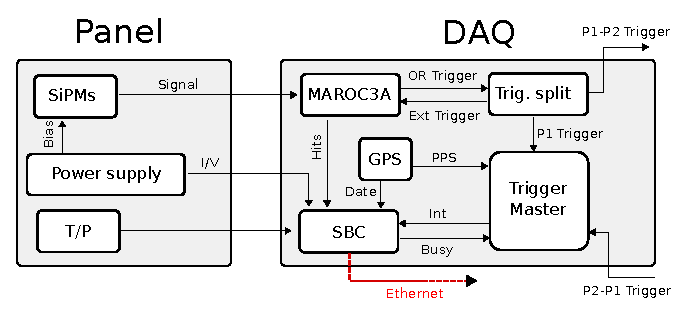
\includegraphics[scale=1.2]{Figures/DAQ.eps}
\caption{Esquema general del sistema de adquisición para un panel centellador.}
\label{DAQ}
\end{figure}

La estampa temporal de los eventos se divide en tres partes: una estampa cada segundo controlada por la señal PPS (Pulse-Per-Second) del GPS, una estampa de 10 ns de resolución establecida por el sistema central de disparo y sincronizada con el PPS y la medición del ToF a una resolución esperada del orden de ps.\\

Los metadatos de temperatura, presión atmosférica y consumo eléctrico se almacenan cada minuto. Finalmente, los datos se almacenan en archivos de una hora de registro cuyo nombre se establece la fecha en el formato Year$\_$ Month$\_$Day$\_$Hour.dat.


\subsection{Caracterización y calibración de los SiPM}

La caracterización del SiPM juega un papel importante ya que permite conocer parámetros como: voltaje de ruptura, , espectro de del foto-electrón, ganancia, conteo oscuro, \textit{cross-talk} y \textit{after-pulse} \cite{sensL2011}. En este caso, se muestra brevemente la metodología de la medición de estos parámetros . 

\subsubsection{Voltaje de ruptura}

El voltaje de ruptura ($V_b$) del SiPM se define como el voltaje de polarización a partir del cual el SiPM funciona en modo Geiger, es decir, el SiPM genera un pulso de corriente cuando un fotón lo impacta. El voltaje de ruptura en el SiPM varia con la temperatura y se determina mediante la curva I-V del SiPM en condiciones de oscuridad.\\

En este caso, las curvas I-V del SiPM se obtuvieron para un rango de temperaturas desde 0$^{\circ}$C hasta 40$^{\circ}$C y una variación del voltaje de polarización de 40V a 60V. Los resultados se muestran en la Fig. \ref{IVSiPM}. Para temperatura ambiente 25$^{\circ}$C, el voltaje de ruptura es 52.3V.

\begin{figure}[h!]
\centering
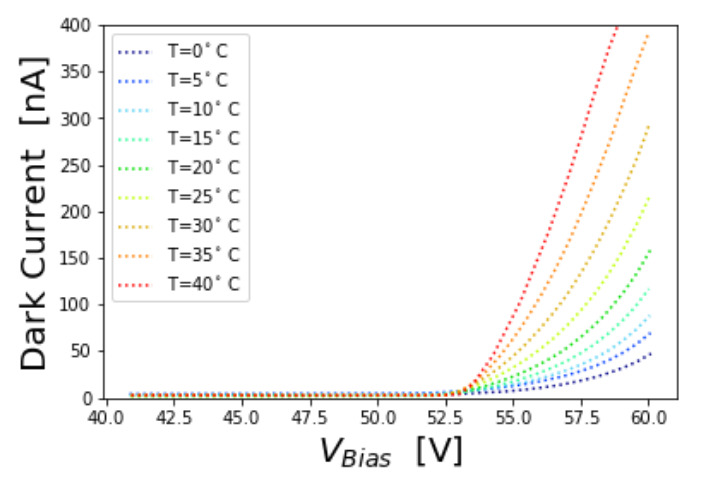
\includegraphics[scale=0.32]{Figures/IVSiPM.jpeg} 
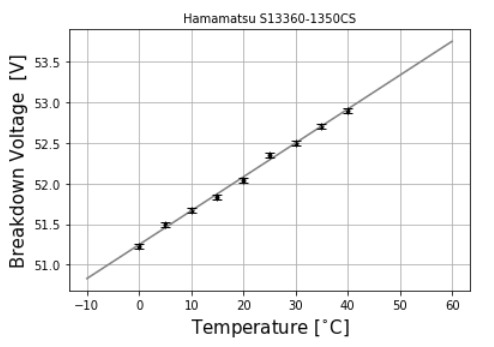
\includegraphics[scale=0.48]{Figures/VbT.jpeg}
\caption{Curvas I-V para el SiPM Hamamatsu 13360-1350CS para temperaturas desde 0$^{\circ}$C hasta 40$^{\circ}$C (izquierda). Dependencia de la temperatura del voltaje de ruptura del SiPM Hamamatsu13360-1350CS (derecha). }
\label{IVSiPM}
\end{figure}

\subsubsection{Espectro de foto-electrón}

El SiPM está formado por una arreglo de foto-diodos de avalancha (APD) conectados en paralelo. La amplitud del pulso de corriente generado es proporcional al número de fotones que inciden sobre él. El espectro de foto-electrón determina el valor equivalente en corriente (o voltaje) de un foto-electrón (p.e.). Este parámetro permite estimar otros parámetros del SiPM como la ganancia, conteo oscuro, \textit{cross-talk} y \textit{after-pulse}.\\

Para obtener dicho espectro, el SiPM fue excitado con una fuente LED pulsada de $\sim$470nm, un ancho de pulso $\sim$9ns, una frecuencia de 500Hz a 25$^{\circ}$C. Los pulsos fueron digitalizados mediante una Red Pitaya con una frecuencia de muestreo de 125 MSPS a 14 bits.\\

Los resultados se exponen el la Fig. \ref{Charge}. El histograma de persistencia se obtuvo con 10000 pulsos. En este caso,  el voltaje de un p.e. estimado es $\sim$13.5mV (izquierda). Por otra parte, el histograma de carga muestra 11 picos de los cuales el primero es el pedestal. La distancia entre picos determina el equivalente en carga de un p.e. $\sim$120ADC.

\begin{figure}[h!]
\centering
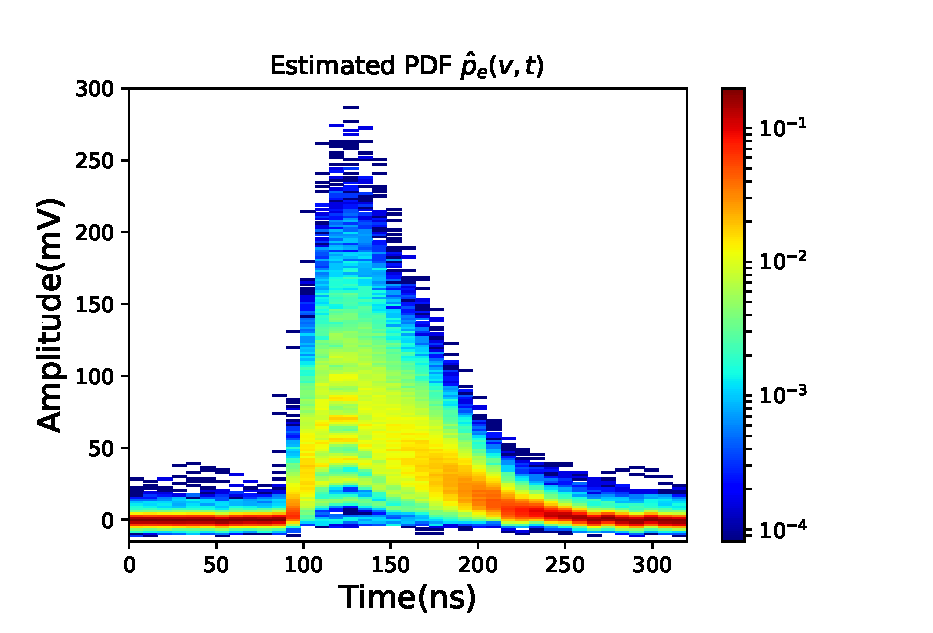
\includegraphics[scale=0.55]{Figures/Pulses} 
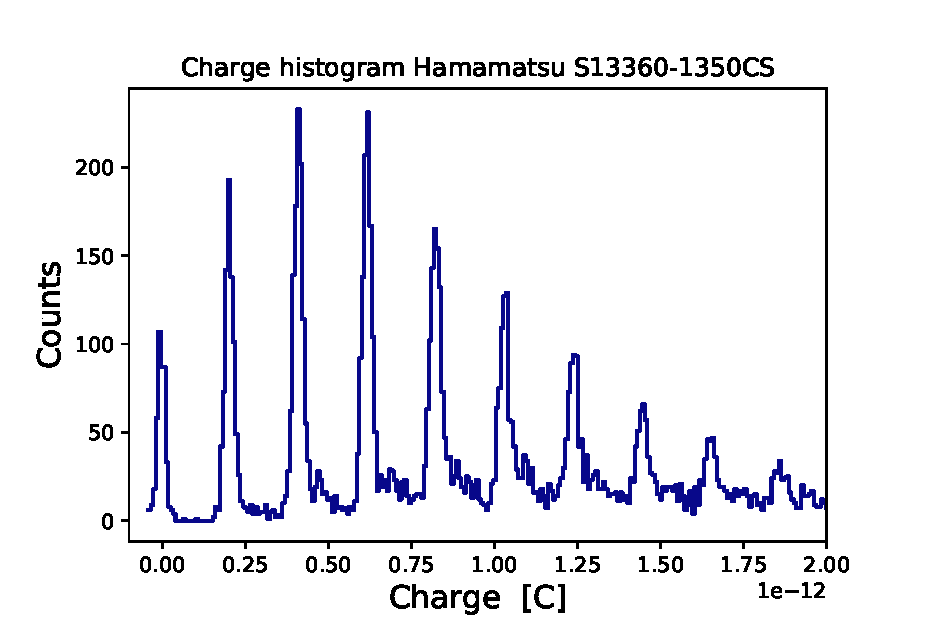
\includegraphics[scale=0.55]{Figures/Charge}
\caption{Pulsos generados por el SiPM 13360-1350CS a 25$^{\circ}$C y 56V (izquierda). Histograma de carga para el SiPM 13360-1350CS a 25$^{\circ}$C y 56V (derecha).}
\label{Charge}
\end{figure}

\subsubsection{Ganancia}

La ganancia del SiPM depende del voltaje de polarización, a medida que el voltaje aumenta, la ganancia también. Para determinar la ganancia del SiPM Hamamatsu 13360-1350CS se obtuvieron tres espectros p.e. para tres aumentos $\Delta$V del voltaje de polarización (1.7V[54V], 2.7V[55V], 3.7V[56V]) a 25$^{\circ}$C ($V_b$ = 52.3V). En la Fig. \ref{Gain}a se muestra la expansión de los espectros p.e. a medida que aumenta $\Delta$V debido al aumento de ganancia. \\

La ganancia se determina dividiendo la diferencia de carga entre picos $\Delta Q$ entre la carga de un electrón $e = 1.6 \times10^{19}$C. Para un $\Delta$V = 3.7V la ganancia es 1.3$\times10^6$ y el cambio de ganancia dependiendo del voltaje es 3.07$\times10^5$/V.

\begin{figure}[h!]
\centering
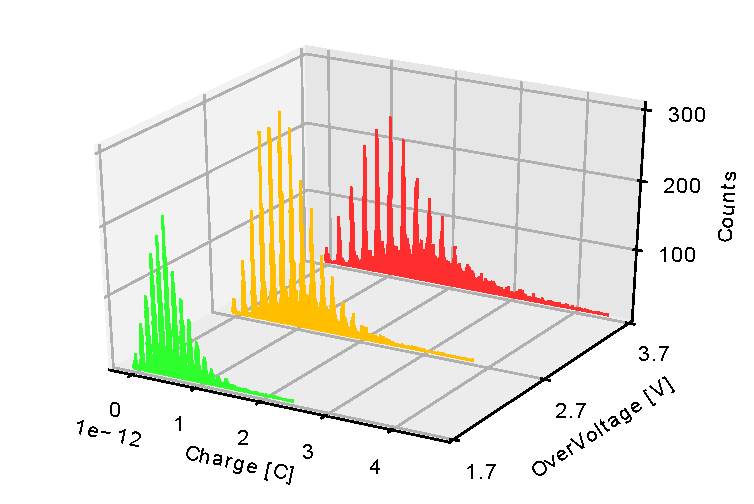
\includegraphics[scale=0.68]{Figures/GainCharge} 
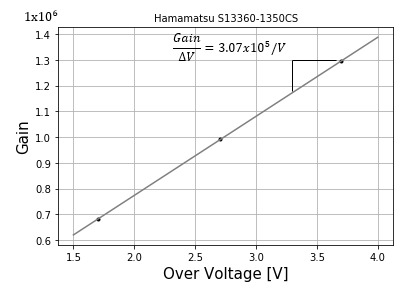
\includegraphics[scale=0.55]{Figures/Gain.jpeg}
\caption{Histograma de carga para el SiPM 13360-1350CS operando a tres sobre voltajes diferentes bajo las mismas condiciones de iluminación a 25$^{\circ}$C (izquierda). Ganancia en función del sobre voltaje a 25$^{\circ}$C (derecha). }
\label{Gain}
\end{figure}

\subsubsection{Conteo oscuro}

La principal fuente de ruido en el SiPM es el conteo oscuro (DCR). Este ocurre debido a electrones térmicamente generados que crean procesos de avalancha. Los pulsos eléctricos resultantes de este proceso son similares a las señales creadas por la incidencia de un fotón. La medición del DCR se debe realizar con el SiPM en condiciones de oscuridad.\\

En este caso, el DCR del SiPM 13360-1350CS se midió para diferentes valores umbrales de discriminación desde 0.1pe hasta 3.1pe a 25$^{\circ}$C como se muestra en la Fig. \ref{DCR}. Para un umbral de 0.5pe el DCR es $\sim$ 2$\times 10^5$ Hz correspondiendo con los valores esperados los cuales varían de 0.9$\times 10^5$ Hz a 2.7$\times 10^5$ Hz.\\

Por otra parte, el DCR disminuye drásticamente a medida que aumenta el nivel del umbral, siendo 1$\times 10^4$ Hz para 1.5pe y  8$\times 10^2$ Hz para 2.5pe. El efecto del DCR a 3.5pe es despreciable.

\begin{figure}[h!]
\centering
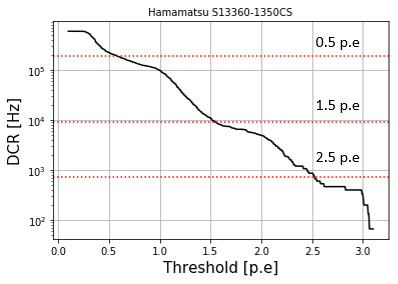
\includegraphics[scale=0.7]{Figures/DCR.jpeg} 
\caption{Frecuencia del conteo oscuro como función del umbral de conteo. }
\label{DCR}
\end{figure}
La prueba anterior permite establecer el valor mínimo que debe tener el umbral de detección de eventos en el sistema de adquisición con el fin de reducir la influencia del ruido por DCR.

\subsubsection{\textit{cross-talk} y \textit{after-pulse}}

Otro componente del ruido del SiPM es el \textit{crosstalk} y el \textit{afterpulse}. El \textit{crosstalk} ocurre cuando los portadores dentro de la avalancha emiten fotones que pueden interactuar con celdas vecinas dentro del SiPM, generando una avalancha en dicha celda. El \textit{crosstalk} se caracteriza por tener amplitudes de 2pe a 3pe.

\begin{figure}[h!]
\centering
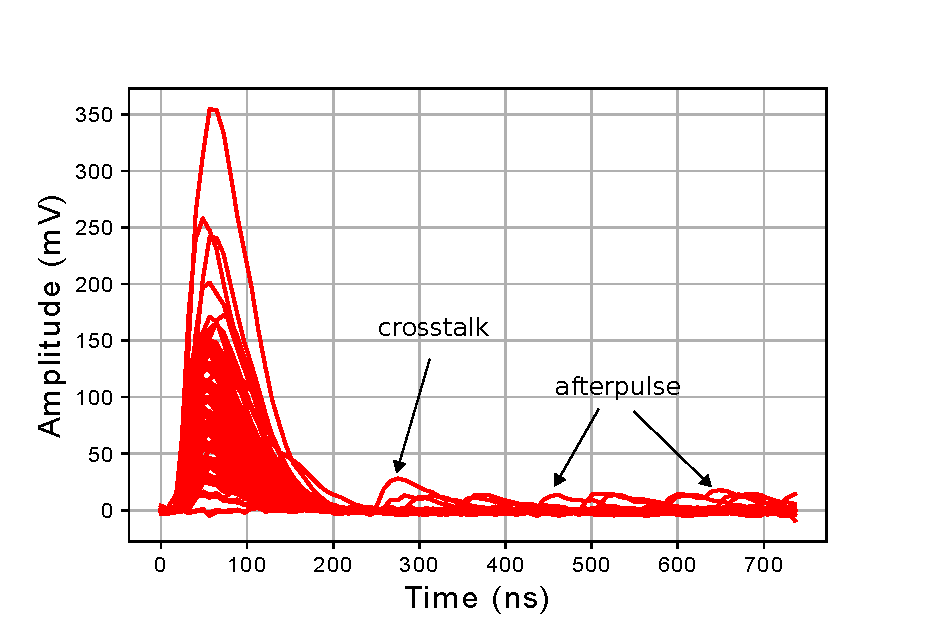
\includegraphics[scale=0.75]{Figures/After}
\caption{Pulsos característicos del \textit{cross-talk} (2pe) y \textit{after-pulse} (1pe) después de un pulso de estimulación lumínica. }
\label{cross}
\end{figure}

Por otra parte, el \textit{afterpulse} es generado por electrones que son atrapados en el material durante el desarrollo de la avalancha, estos electrones se liberan pocos nanosegundos después creando una nueva avalancha, y por ende un pulso consecutivo. En la Fig. \ref{cross} se muestra un ejemplo de \textit{crosstalk} y \textit{afterpulse}.

Para la estimación de estas dos fuentes de ruido se estimuló el SiPM mediante la fuente pulsada de luz a 500 Hz. En este caso el \textit{crosstalk} es $\sim$ 0.3$\%$ y el \textit{afterpulse} $\sim$ 3.4$\%$.

\subsection{Caracterización de las barras centelladoras}

El número de fotones que llegan al SiPM depende del lugar donde interactúa la partícula con el centellador \cite{Calderon2019}. Debido a la longitud de atenuación del centellador (5.5 cm) los fotones son canalizados hasta el SiPM a través de la fibra óptica.

\begin{figure}[h!]
\centering
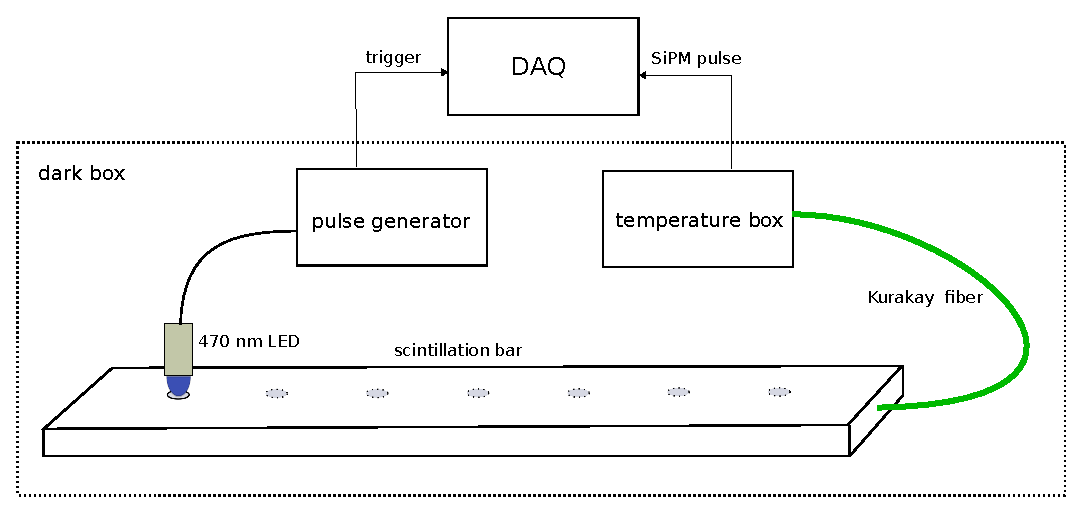
\includegraphics[scale=0.75]{Figures/BarAtt.eps}
\caption{Montaje experimental para la medición de la atenuación y el retardo en la señal registrada por los SiPM dependiendo de la distancia al punto de interacción en la barra centelladora.}
\label{AtTest}
\end{figure}

Para estimar la atenuación del sistema centellador-fibra, se crean 23 puntos de estimulación en el centellador con un paso de 5cm. Cada punto es estimulado con la fuente pulsada de 470nm. La señal generada por el SiPM es digitalizada a 14 bits y 125 MSPS. El montaje del experimento se muestra en la Fig. \ref{AtTest}.\\

Para cada punto de prueba se adquirieron 1000 puntos. A una distancia de x=120 cm la amplitud de la señal se atenúa hasta un 70$\%$ de la amplitud a x=0 cm. Dicho comportamiento de atenuación debe tenerse en cuenta durante la calibración de los paneles centelladores ya que en el píxel más alejado (x=120 cm, y=120 cm) de la zona donde se ubican los SiPM, la atenuación será 49$\%$.\\

Por otra parte, también se caracteriza el tiempo de retardo de la señal generada en el centellador dependiendo del punto de estimulación. Comparando tres puntos de estimulación en la barra centelladora (5 cm, 55 cm y 115 cm) se observa un retardo de 8.5 ns entre los puntos extremos ($\Delta x =$ 110 cm), es decir, los fotones recorren 1 cm en 77.2 ps. En la Fig. \ref{AttCur} se observan los tiempos de arribo de la señal al SiPM dependiendo del punto de interacción y la curva de atenuación del centellador.

\begin{figure}[h!]
\centering
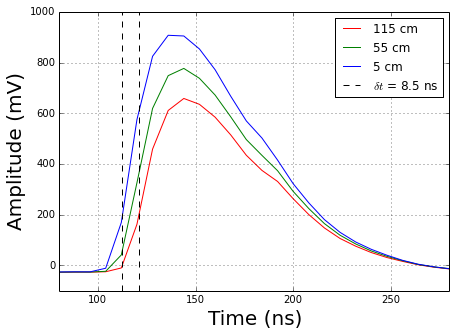
\includegraphics[scale=0.5]{Figures/arrivT.png}
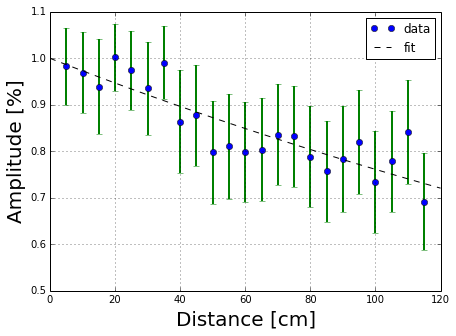
\includegraphics[scale=0.5]{Figures/Attenuation.png}
\caption{Retardo temporal de la señal del SiPM para una estimulación a 115 cm, 55 cm y 5 cm (izquierda). Curva de atenuación de la señal del SiPM dependiendo de la distancia de la estimulación (derecha).}
\label{AttCur}
\end{figure}

\subsection{Calibración de los paneles centelladores y hodoscopio}

El desempeño de los paneles centelladores es evaluado mediante el registro de flujo de muones atmosféricos. En este caso, los paneles registraron el flujo durante 15 horas continuas. Con los datos obtenidos se evaluó la varianza del flujo registrado por cada una de las 60 barras centelladores que componen cada panel. En la Fig. \ref{Bar_var} se observan los resultados obtenidos donde las barras detectan un promedio de 836 eventos/hora con una variabilidad de 96.3 eventos/h.

\begin{figure}[h!]
\centering
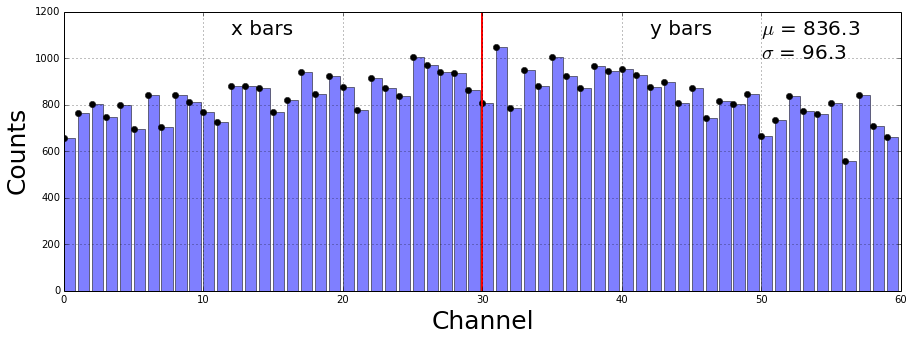
\includegraphics[scale=0.5]{Figures/hist2.png}
\caption{Histograma de eventos registrados por las 60 barras de un panel centellador durante una hora de registro. La línea roja separa las barras verticales y horizontales que componen la matriz de píxeles.}
\label{Bar_var}
\end{figure}

Por otra parte, los paneles centelladores presentan una atenuación debido a la combinación de la atenuación de las barras que lo componen. En la Fig. \ref{Pan_At} se muestra el histograma de conteo de los eventos registrados en 15 horas. En este caso, los píxeles más alejados (29,29) de la posición de los SiPM presentan un número de eventos menor en comparación al más cercano (0,0). La atenuación esperada en cada píxel se estima como la multiplicación de las atenuaciones de la barra-x y la barra-y que componen dicho píxel. El histograma de eventos en el panel permite además evaluar problemas en las barras centelladoras. En este caso podemos ver un mal funcionamiento de la barra-y 26 y 20.

\begin{figure}[h!]
\centering
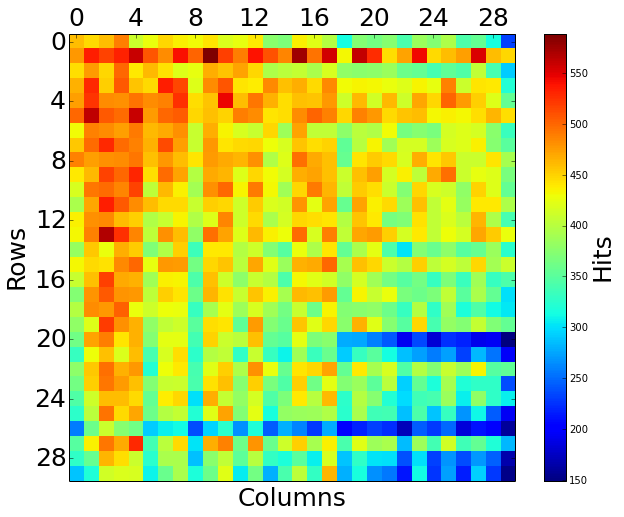
\includegraphics[scale=0.5]{Figures/P2_15h.png}
\caption{Histograma de eventos registrados por un panel centellador durante 15 horas. La atenuación del número de eventos registrados se incrementa diagonalmente desde la esquina superior-izquierda (0,0) a la esquina inferior-derecha (29,29).}
\label{Pan_At}
\end{figure}


\section{Diseño electrónico y calibración del WCD}

Para eliminar las fuentes de ruido que influyen en la técnica de muografía se emplearán sistemas de identificación de partículas. La diferenciación entre los eventos generados por la componente suave de las EAS (electrones y positrones) y los muones se realizará mediante la medición de la pérdida de energía de estas partículas cargadas en un WCD. El WCD de MuTe se diseñará y construirá teniendo en cuenta la experiencia previa del proyecto LAGO\footnote{http://lagoproject.net/} (por sus siglas en inglés Latin American Giant Observatory) del cual nuestro grupo hace parte.\\

Los detalles técnicos y resultados preliminares de las actividades relacionadas con este objetivo se muestran a continuación.\\

\textbf{Actividades y resultados preliminares}\\

\subsection{Diseño del WCD}

El WCD está compuesto por un tanque cúbico de aluminio con 120 cm de lado, recubierto internamente con Tyvek para aumentar la eficiencia en la detección de los fotones Cherenkov. El WCD esta lleno de agua purificada con 28 ppm de cloro. El dispositivo sensor es el tubo foto-multiplicador (PMT) Hamamatsu R5912 de 8". El PMT tiene una eficiencia cuática 22$\%$ a 390 nm, una ganancia de hasta 10$^7$ con un voltaje de polarización de 1800 V y un tiempo subida en el ánodo de 3.8 ns. La estructura del WCD se muestra en la Fig. \ref{WCD}.\\

\begin{figure}[h!]
\centering
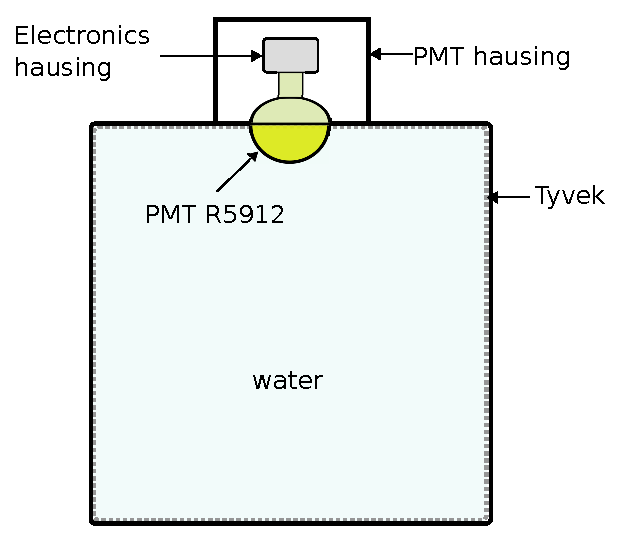
\includegraphics[scale=1]{Figures/WCD.eps}
\caption{Estructura mecánica del WCD de MuTe.}
\label{WCD}
\end{figure}

\subsection{Diseño del sistema de adquisición del WCD}

El sistema de adquisición del WCD registra las señales del ánodo y del último dínodo del PMT. Para aumentar el rango de medida la señal del dínodo es amplificada en un factor 20. La señales son digitalizadas por un ADC de 10 bits con una frecuencia de muestreo de 40 MHz. Cuando un evento supera el umbral de detección la forma de onda del pulso es almacenada en un vector de 12 muestras (300 ns).\\

Cada evento tiene una estampa temporal de 25 ns de resolución, la cual es sincronizada con la señal PPS del GPS. Los datos son transmitidos por protocolo UART a un SCB (Cubieboard II) que los almacena en archivos de una hora de registro junto con metadatos de temperatura y presión atmosférica.\\

Los eventos en coincidencia con el hodoscopio se registran a través de la señal de disparo (NIM Trigger). El esquema general del sistema de adquisición se muestra en la Fig. \ref{WCDDAQ}.

\begin{figure}[h!]
\centering
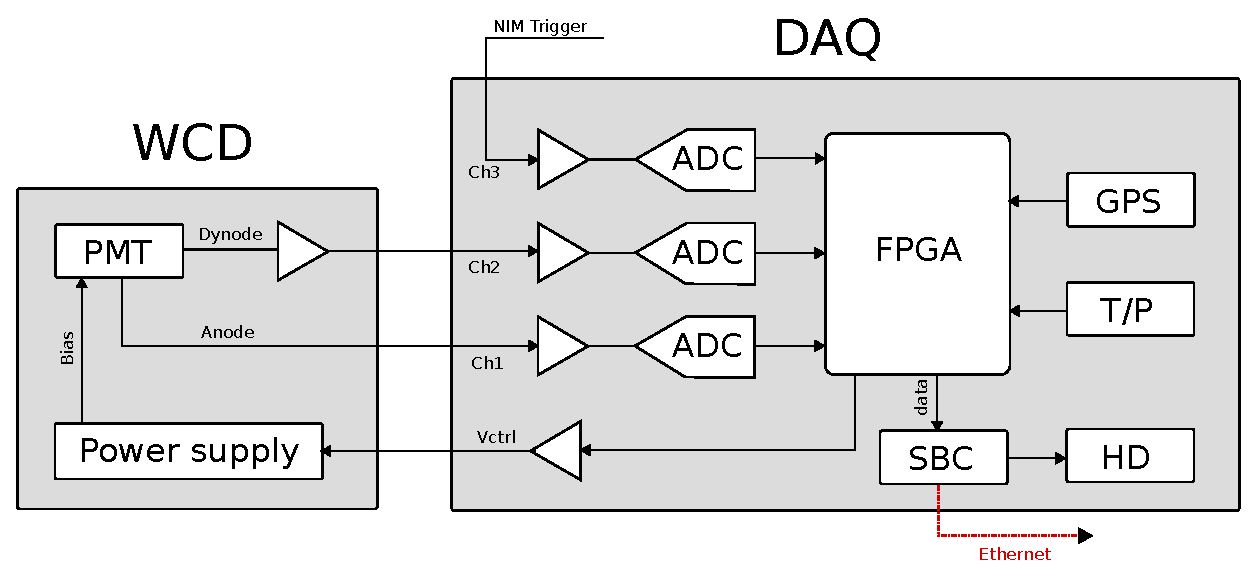
\includegraphics[scale=0.7]{Figures/WCDDAQ.eps}
\caption{Esquema general del sistema de adquisición del WCD}
\label{WCDDAQ}
\end{figure}

\subsection{Calibración del WCD}

La calibración del WCD se compone de dos pasos: la calibración del voltaje óptimo de operación del PMT y la calibración de la energía depositada por las partículas cargadas.\\

\subsubsection{Calibración del voltaje de polarización}

Para realizar la calibración del voltaje óptimo se registran la tasa de eventos $\Phi$ del fondo de rayos cósmicos a diferentes voltajes de polarización y diferentes umbrales de discriminación \cite{Leon2017}.\\

La calibración del WCD consistió en hacer un barrido de voltajes de polarización desde 740 V a 1450 V con pasos de 102 V para tres diferentes umbrales de discriminación: 110 mV, 160 mV y 210 mV. Para cada caso, se registraron 10 minutos de datos. En la Fig. \ref{plateau} se muestra la tasa de eventos registrados dependiendo del voltaje de polarización para 110 mV (negro), 160 mV (azul) y 210 mV(rojo).\\

En las curvas se puede observar una región de baja pendiente llamada \textit{plateau}. En esta región se ubica el punto óptimo de operación del PMT. Para hallar dicho punto se desarrolló un método automático que se basa en la minimización de la derivada respecto al voltaje de la tasa de detección.\\

Por lo tanto, el voltaje óptimo de operación $V^{\ast}_b$ es definido como:

\begin{equation}
V^{\ast}_b =  \textrm{argmin} \frac{\textrm{d}\Phi}{\textrm{d} V} 
\end{equation}

\begin{figure}[h!]
\begin{center}
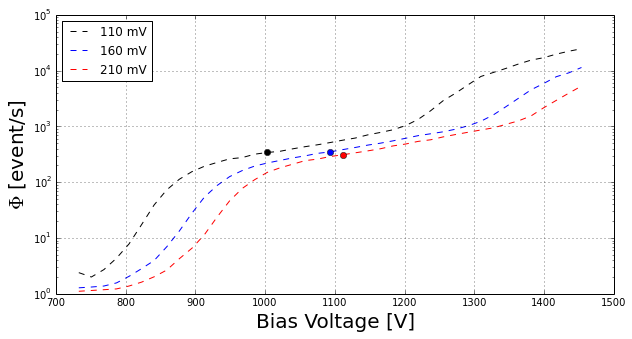
\includegraphics[width=0.8\textwidth]{Figures/WCDCalibrated}
\caption{Tasa de eventos detectada para voltajes de polarización desde 740 V hasta 1450 V para un umbral de 110 mV (negro), 160 mV (azul) y 210 mV (rojo).}
\label{plateau}
\end{center}
\end{figure}

\begin{figure}[h!]
\begin{center}
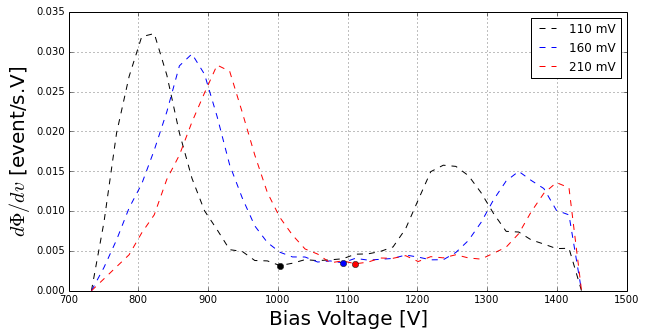
\includegraphics[width=0.8\textwidth]{Figures/OptimumPoint}
\caption{Voltaje óptimo de polarización del WCD para un umbral de 110 mV (negro), 160 mV (azul) y 210 mV (rojo).}
\label{OptimumWCD}
\end{center}
\end{figure}

En la Fig. \ref{OptimumWCD} se observan los voltajes de polarización hallados para los tres casos evaluados, 1000 V (110 mV), 1096 V (160 mV) y 1109 V (210 mV). 

\subsubsection{Calibración de la respuesta a la energía depositada}

Un punto importante es la calibración de la respuesta del WCD a la energía depositada de las partículas cargadas que lo atraviesan. Para ello se genera un histograma de carga desde los datos recolectados. Este histograma se basa en estimar el área bajo la curva de cada pulso registrado y sus unidades son ADC.bin.\\

En la Fig. \ref{ChargeHis} se muestra el histograma de carga para una hora de datos. Se pueden observar dos jorobas, la más pronunciada se debe a la componente electromagnética de las EAS, es decir, electrones, positrones y gammas. Por otra parte, la segunda joroba pertenece a la componente muónica de las EAS y su media se denomina VEM.\\

\begin{figure}[h!]
\begin{center}
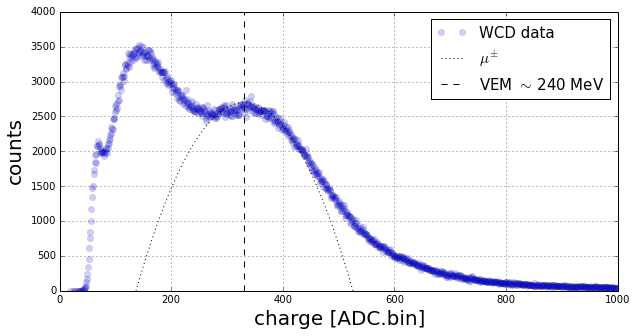
\includegraphics[width=0.8\textwidth]{Figures/dEdxCal}
\caption{Histograma de carga para una hora de datos. El VEM se ubica en 331.4 ADC.bin.}
\label{ChargeHis}
\end{center}
\end{figure}

El VEM (equivalente a un muón vertical) es la pérdida de energía que genera un muón cuando ingresa ortogonalmente por la parte superior del WCD. Teniendo en cuenta que un muón pierde alrededor de 2 MeV/cm en el agua, y que la altura del WCD es de 120 cm, entonces la pérdida de energía total de un muón que atraviese el WCD ortogonalmente es de 240 MeV.\\

Teniendo en cuenta lo anterior, la pérdida de energía dependiendo de la carga depositada se expresa como:

\begin{equation}
    E_{loss} =  (\text{ADC.bin})\frac{240 \text(MeV)}{ \text{VEM}_q(\text{ADC.bin})}
\end{equation}

donde $\text{VEM}_q$ es el valor del VEM en el histograma de carga, en este caso 331.4 ADC.bin.

\section{Diseño y calibración del sistema ToF}

Para filtrar los muones de baja energía ($<$ 1 GeV) \cite{Bozza2017} que componen una de las principales fuentes de contaminación en muografía se desarrollará un sistema de medición del tiempo de vuelo de las partículas cargadas que cruzan el hodoscopio. En este caso, se diseñará una arquitectura basada en líneas de retardo y un oscilador de anillo implementados en una FPGA Spartan 6 de Xilinx. Finalmente, el sistema ToF será calibrado y validado mediante la comparación de mediciones con el sistema ToF comercial TDC7200 de Texas Instruments.\\

Los detalles técnicos y resultados preliminares de las actividades relacionadas con este objetivo se muestran a continuación.\\

\textbf{Actividades y resultados preliminares}\\

\subsection{Diseño del sistema  TDC}

El sistema ToF se basa en un TDC (Time-to-Digital Converter) compuesto de una línea de retardo de 100 etapas (contador fino) y un oscilador de anillo para ampliar el rango de medición (contador grueso). Ver Fig. \ref{Arch}.\\

\begin{figure}[h!]
\begin{center}
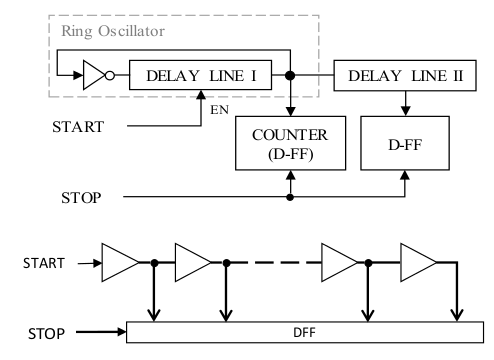
\includegraphics[width=0.6\textwidth]{Figures/Architecture}
\caption{Esquema del sistema de medición del tiempo de vuelo compuesto por una línea de retardo (contador fino) y un oscilador de anillo (contador grueso) (arriba). Esquema básico de la línea de retardo (abajo).}
\label{Arch}
\end{center}
\end{figure}

El TDC se implemento en una FPGA Spartan 6. Las etapas de retardo se diseñaron usando el módulo CARRY4 el cual está compuesto de 4 multiplexores los cuales se ubicaron de manera consecutiva para garantizar una respuesta lineal del TDC.\\

\subsection{Calibración del sistema  TDC}

La calibración del contador fino se realizó inyectando una señal cuadrada de 200 Hz desde un generador de señales (Tektronix AFG1022) y observando su retraso después de pasar secciones de 10 etapas. La curva de calibración obtenida se puede ver en la Fig. \ref{loc}. El retardo promedio por etapa es de 40$\pm$26 ps.\\

\begin{figure}[h!]
\begin{center}
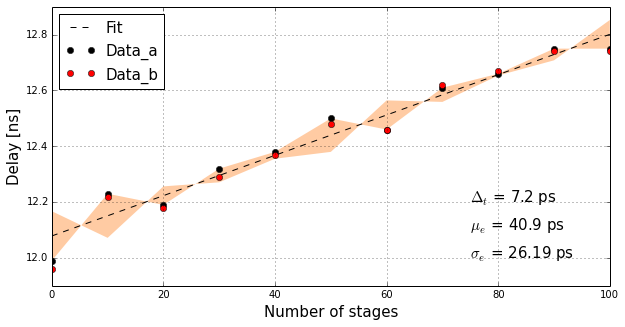
\includegraphics[width=0.7\textwidth]{Figures/ToF_delay}
\caption{Retardo de la señal dependiendo del número de etapas ubicadas en dos regiones distintas de la FPGA (a y b)}
\label{loc}
\end{center}
\end{figure}

El contador grueso se compone de una línea de retardo de 100 etapas retroalimentada con el inverso de su salida. La retroalimentación es controlada a través de un multiplexor.

\begin{figure}[h!]
\begin{center}
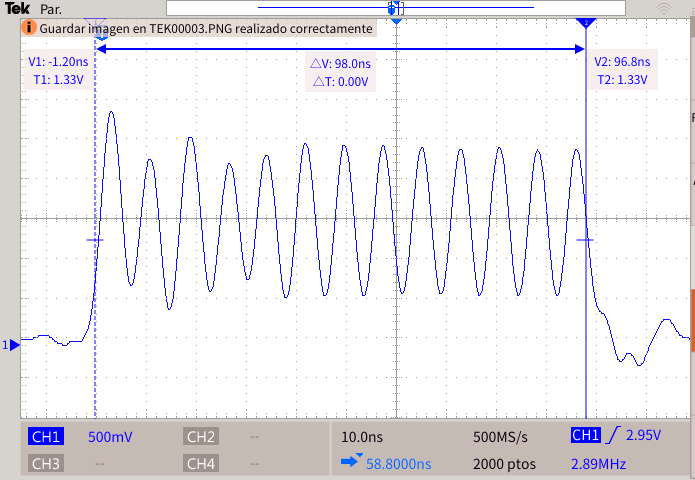
\includegraphics[width=0.6\textwidth]{Figures/Ringwaves}
\caption{Salida del oscilador de anillo para un retraso entre la señal \textbf{Start} y \textbf{Stop} de 100 ns.}
\label{waves}
\end{center}
\end{figure}

Teniendo que cada etapa tiene un retardo de 40$\pm$26 ps, el período de oscilación esperado para 100 etapas es $\sim$8 ns. En la Fig. \ref{waves} se muestra la salida del oscilador de anillo para un retrazo entre la señal \textbf{Start} y \textbf{Stop} de 100 ns. En este caso, se registran 13 oscilaciones, es decir, el periodo de oscilación es $\sim$7.7ns.\\



Para calibrar el contador grueso se ingresaron retardos controlados desde 0 ns a 90 ns medidos paralelamente con un osciloscopio Textronix TDS2004B. En la Fig. \ref{CalCoarse} se muestra el conteo de los picos de oscilación dependiendo del tiempo de retardo entre \textbf{Start} y \textbf{Stop}. La linealidad de la etapa disminuye a medida que el rango de medición aumenta, la región óptima de medición se ubica de 0 ns a 60 ns. Además, el desempeño del sistema TDC implementado en MuTe será comparado con el TDC7200 de Texas Instruments.

\begin{figure}[h!]
\begin{center}
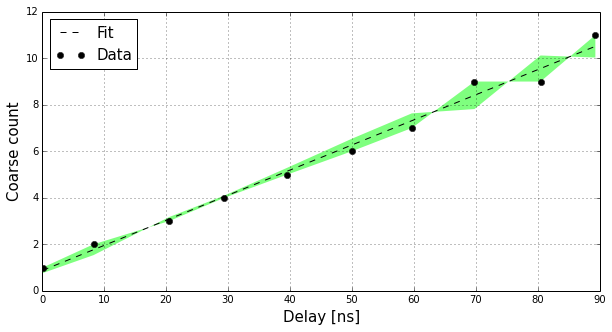
\includegraphics[width=0.7\textwidth]{Figures/Cal_coarse}
\caption{Curva de calibración del contador grueso del sistema ToF.}
\label{CalCoarse}
\end{center}
\end{figure}

Los datos del ToF se transmiten a la SBC de cada panel mediante un protocolo I2C en una trama compuesta por dos valores: el contador fino y el contador grueso.

\section{Calibración del MuTe y pruebas de estabilidad}

Una vez se calibra el hodoscopio y el WCD, se procederá a la calibración conjunta del MuTe. La calibración se hará mediante la detección de eventos provenientes del fondo de rayos cósmicos atmosféricos y el análisis de datos.\\

El MuTe registrará eventos continuamente durante varios días junto con los metadatos de temperatura, presión atmosférica, consumo eléctrico y estampas temporales de los paneles centelladores y el WCD. Los datos serán analizados evaluando los siguientes aspectos:

\begin{itemize}
    \item Funcionamiento total de las barras centelladoras en busca de fallas por transporte
    \item Posibles variaciones del flujo registrado por los paneles de centelleo y el WCD debido a variaciones de temperatura o presión atmosférica
    \item Excesos en el pico electromagnético del WCD debido a contaminación por fotones
    \item Correcta transmisión de los datos desde los paneles de centelleo al disco duro central
    \item Evaluación de coincidencias entre el hodoscopio y el WCD
    \item Corrección temporal de los eventos teniendo en cuenta los retrasos por las líneas de transmisión
    \item Imágenes muongráficas con y sin las componentes generadoras de ruido
    
\end{itemize}

Finalmente, el detector se dejará adquiriendo de manera constante hasta que se necesite trasladar a otro sitio.
